\documentclass[final, 12pt]{beamer}
\usepackage[T1]{fontenc}
\usepackage[utf8]{luainputenc}
\usepackage{lmodern}
\usepackage[size=custom, width=120,height=90, scale=1.15]{beamerposter}
\usetheme{gemini}
\usecolortheme{uoft}
\usepackage{graphicx}
\usepackage{booktabs}
\usepackage{tikz}
\usepackage{pgfplots}
\pgfplotsset{compat=1.14}
\usepackage{anyfontsize}
\usepackage{subfig}
\usepackage[font=normalsize,labelfont=bf]{caption}
% ====================
% Lengths
% ====================

% If you have N columns, choose \sepwidth and \colwidth such that
% (N+1)*\sepwidth + N*\colwidth = \paperwidth
\newlength{\sepwidth}
\newlength{\colwidth}
\newlength{\smallcolwidth}
\newlength{\bigcolwidth}

\setlength{\sepwidth}{0.025\paperwidth}
\setlength{\colwidth}{0.3\paperwidth}
\setlength{\smallcolwidth}{0.225\paperwidth}
\setlength{\bigcolwidth}{0.45\paperwidth}

\newcommand{\separatorcolumn}{\begin{column}{\sepwidth}\end{column}}
\title{Optimizing Aircraft Engine RUL Prediction with Bayesian-Enhanced Interpretable ML and SHAP}
\author{Juan Pablo Echeagaray González \\ \textit{School of Engineering and Sciences}}
% ====================
% Logo (optional)
% ====================

% use this to include logos on the left and/or right side of the header:
% Left: institution
 \logoleft{
\includegraphics[height=10cm]{logos/ING.png}}

\begin{document}

\begin{frame}[t]
\begin{columns}[t]
\separatorcolumn

\begin{column}{\smallcolwidth}

    \begin{block}{Introduction}

        \begin{itemize}
            \item \textbf{Precision Planning:} Optimizes maintenance schedules, minimizing costs while ensuring maximum efficiency.
            \item \textbf{Elevated Performance:} Enhances operational efficiency and security, elevating the standards for engine maintenance.
            \item \textbf{Sustainability in Practice:} Fosters sustainable operations, aligning with eco-conscious practices for long-term reliability.
        \end{itemize}

    \end{block}

    \begin{block}{Problem Statement}

        The main goal is to estimate the remaining useful life (RUL) of a fleet of turbofan engines under challenging conditions, characterized by high variability and multiple failure modes.
        \begin{itemize}
            \item \textbf{Efficient Modelling:} need for lower cost models
            \item \textbf{Model Interpretability:} understand predictions in critical scenarios
            \item \textbf{Confidence and prediction intervals:} provide measures of uncertainty
        \end{itemize}

        \begin{figure}
            \centering
            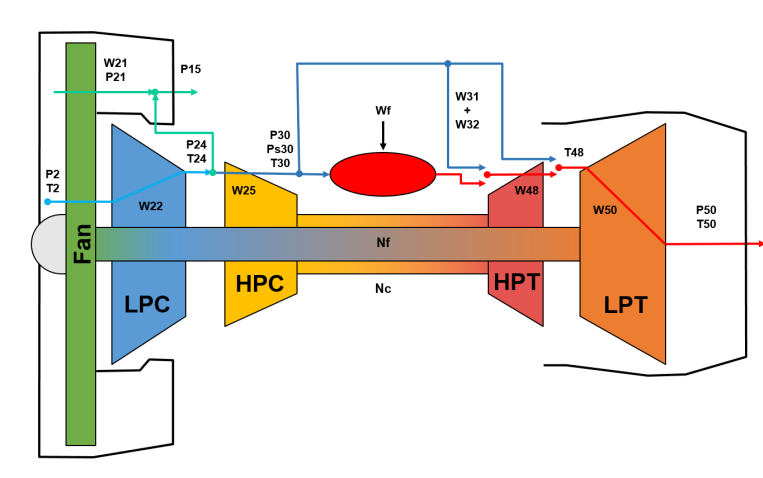
\includegraphics[width=0.8\textwidth]{figures/cmapss_turbofan.png}
            \caption{Schematics of a turbofan engine}
        \end{figure}

        The effectiveness of the proposed model is measured with the PHMAP 2021 Data Challenge Loss function \cite{chao2021phm}:

        \begin{equation} \label{eqn:phmap_loss}
            \begin{gathered}
                RMSE = \sqrt{\frac{1}{m}\sum_{i=1}^{m} (y_i - \hat{y}_i)^{2}} \\
                NASA = \frac{1}{m}\sum_{i=1}^{m} \left[\exp (\alpha \cdot (y_i - \hat{y}_i)) - 1\right]\\
                \alpha = \begin{cases}
                    \frac{-1}{10} & \text{if } y_i - \hat{y}_i \leq 0 \\
                    \frac{1}{13} & \text{if } y_i - \hat{y}_i > 0
                \end{cases}  \\
                \mathcal{L}(y, \hat{y}) = \frac{1}{2} \left(RMSE + NASA\right) \\
            \end{gathered}
        \end{equation}

    \end{block}

\end{column}

\separatorcolumn

\begin{column}{\bigcolwidth}

    \begin{block}{Methodology}

        \begin{figure}
            \centering
            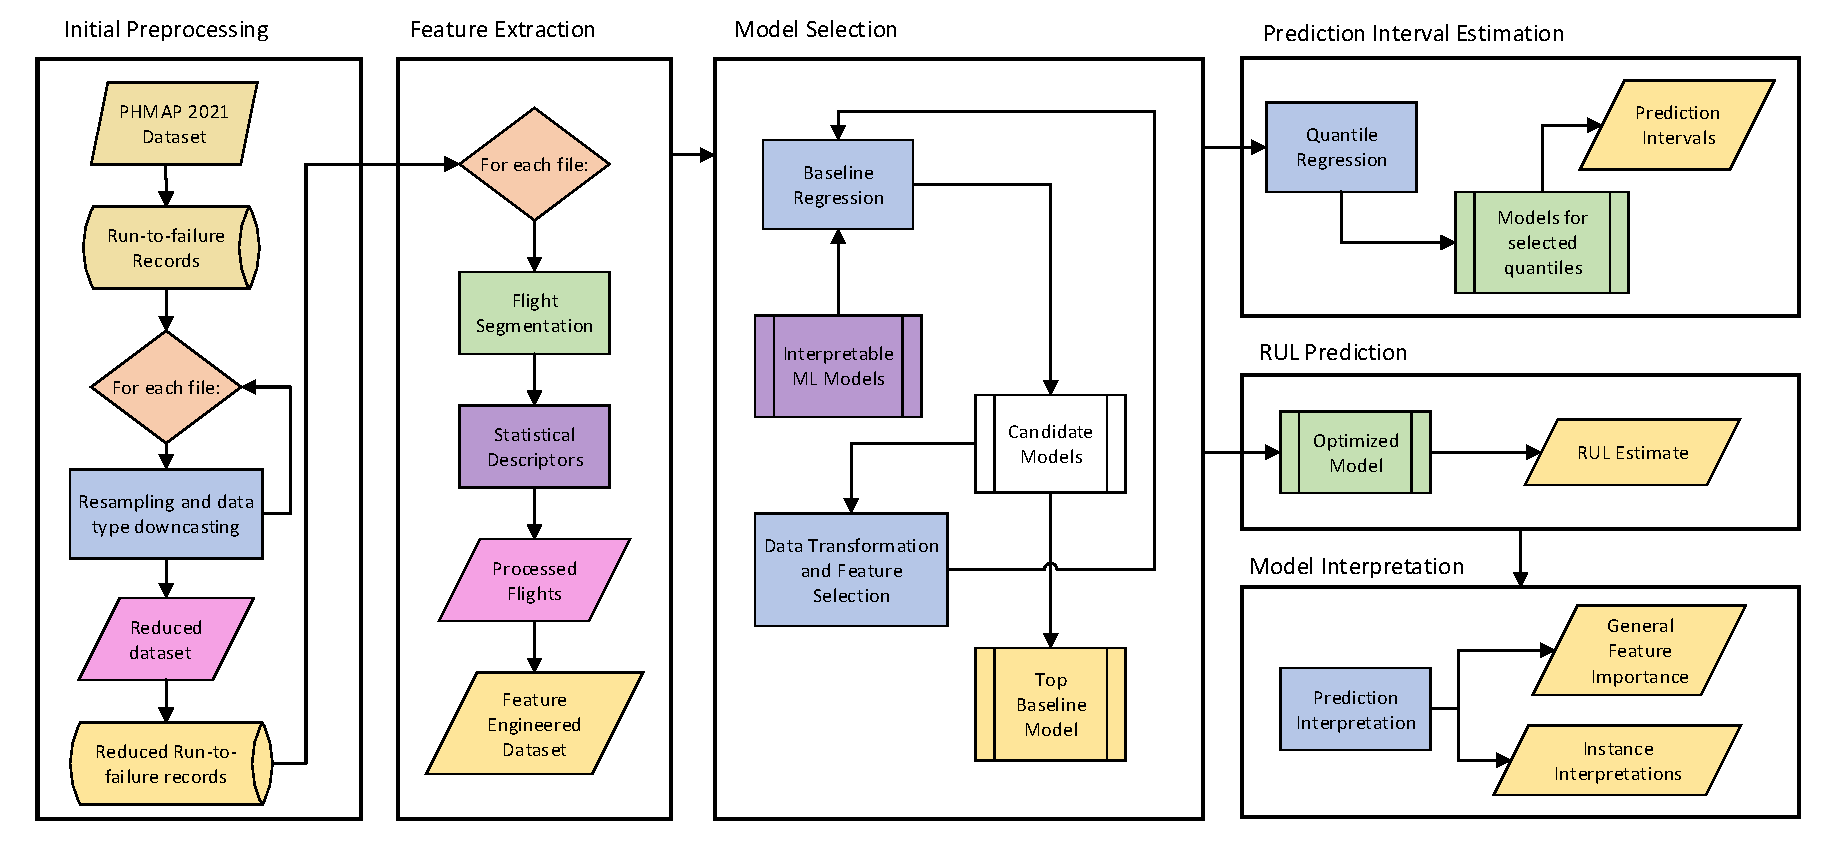
\includegraphics[width=\textwidth]{figures/research_diagram.pdf}
            \caption{Proposed methodology}
        \end{figure}

    \end{block}

    \begin{block}{Results}

        \begin{itemize}
            \item \textbf{Model Selection and Optimization:} Employed diverse models such as Linear Regression, SVM, and gradient boosting, with XGBoost chosen for its rapid learning and potential GPU integration after the dominance of gradient boosting.
            \item \textbf{Enhanced Model Performance:} Used \textit{Tree-Structured Parzen Estimators} \cite{bergstra2011algorithms} to optimize XGBoost \cite{guo2019xgboost}, achieving superior performance to default settings after \textit{500 iterations} across all models.
        \end{itemize}

        \begin{figure}
            \centering
            \subfloat[\centering RUL estimates and prediction intervalss]{{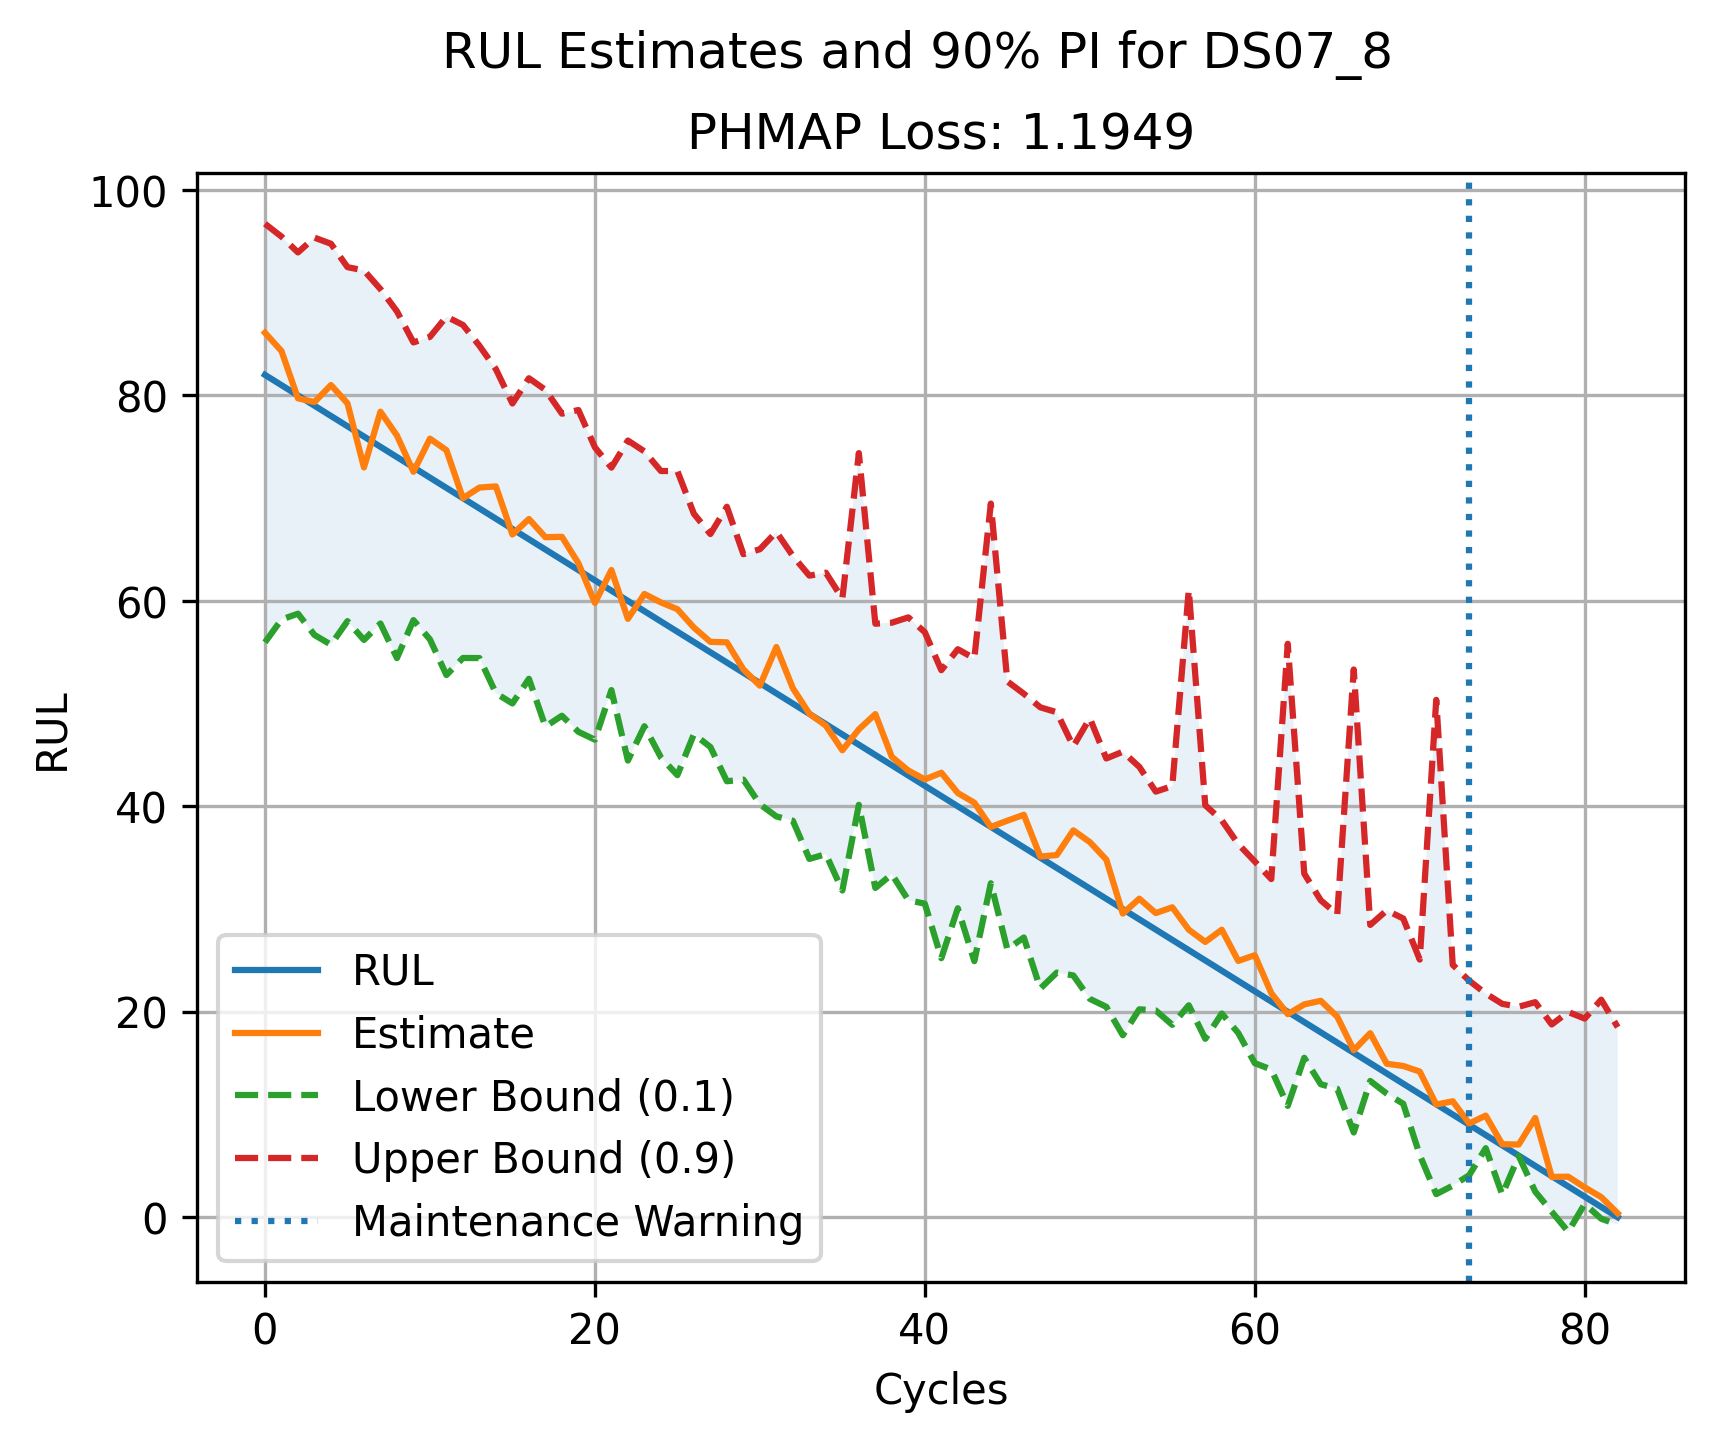
\includegraphics[scale=1.7]{figures/preds_DS07_8.png}}}
            \qquad
            \subfloat[\centering Distribution of Shapley Values per feature]{{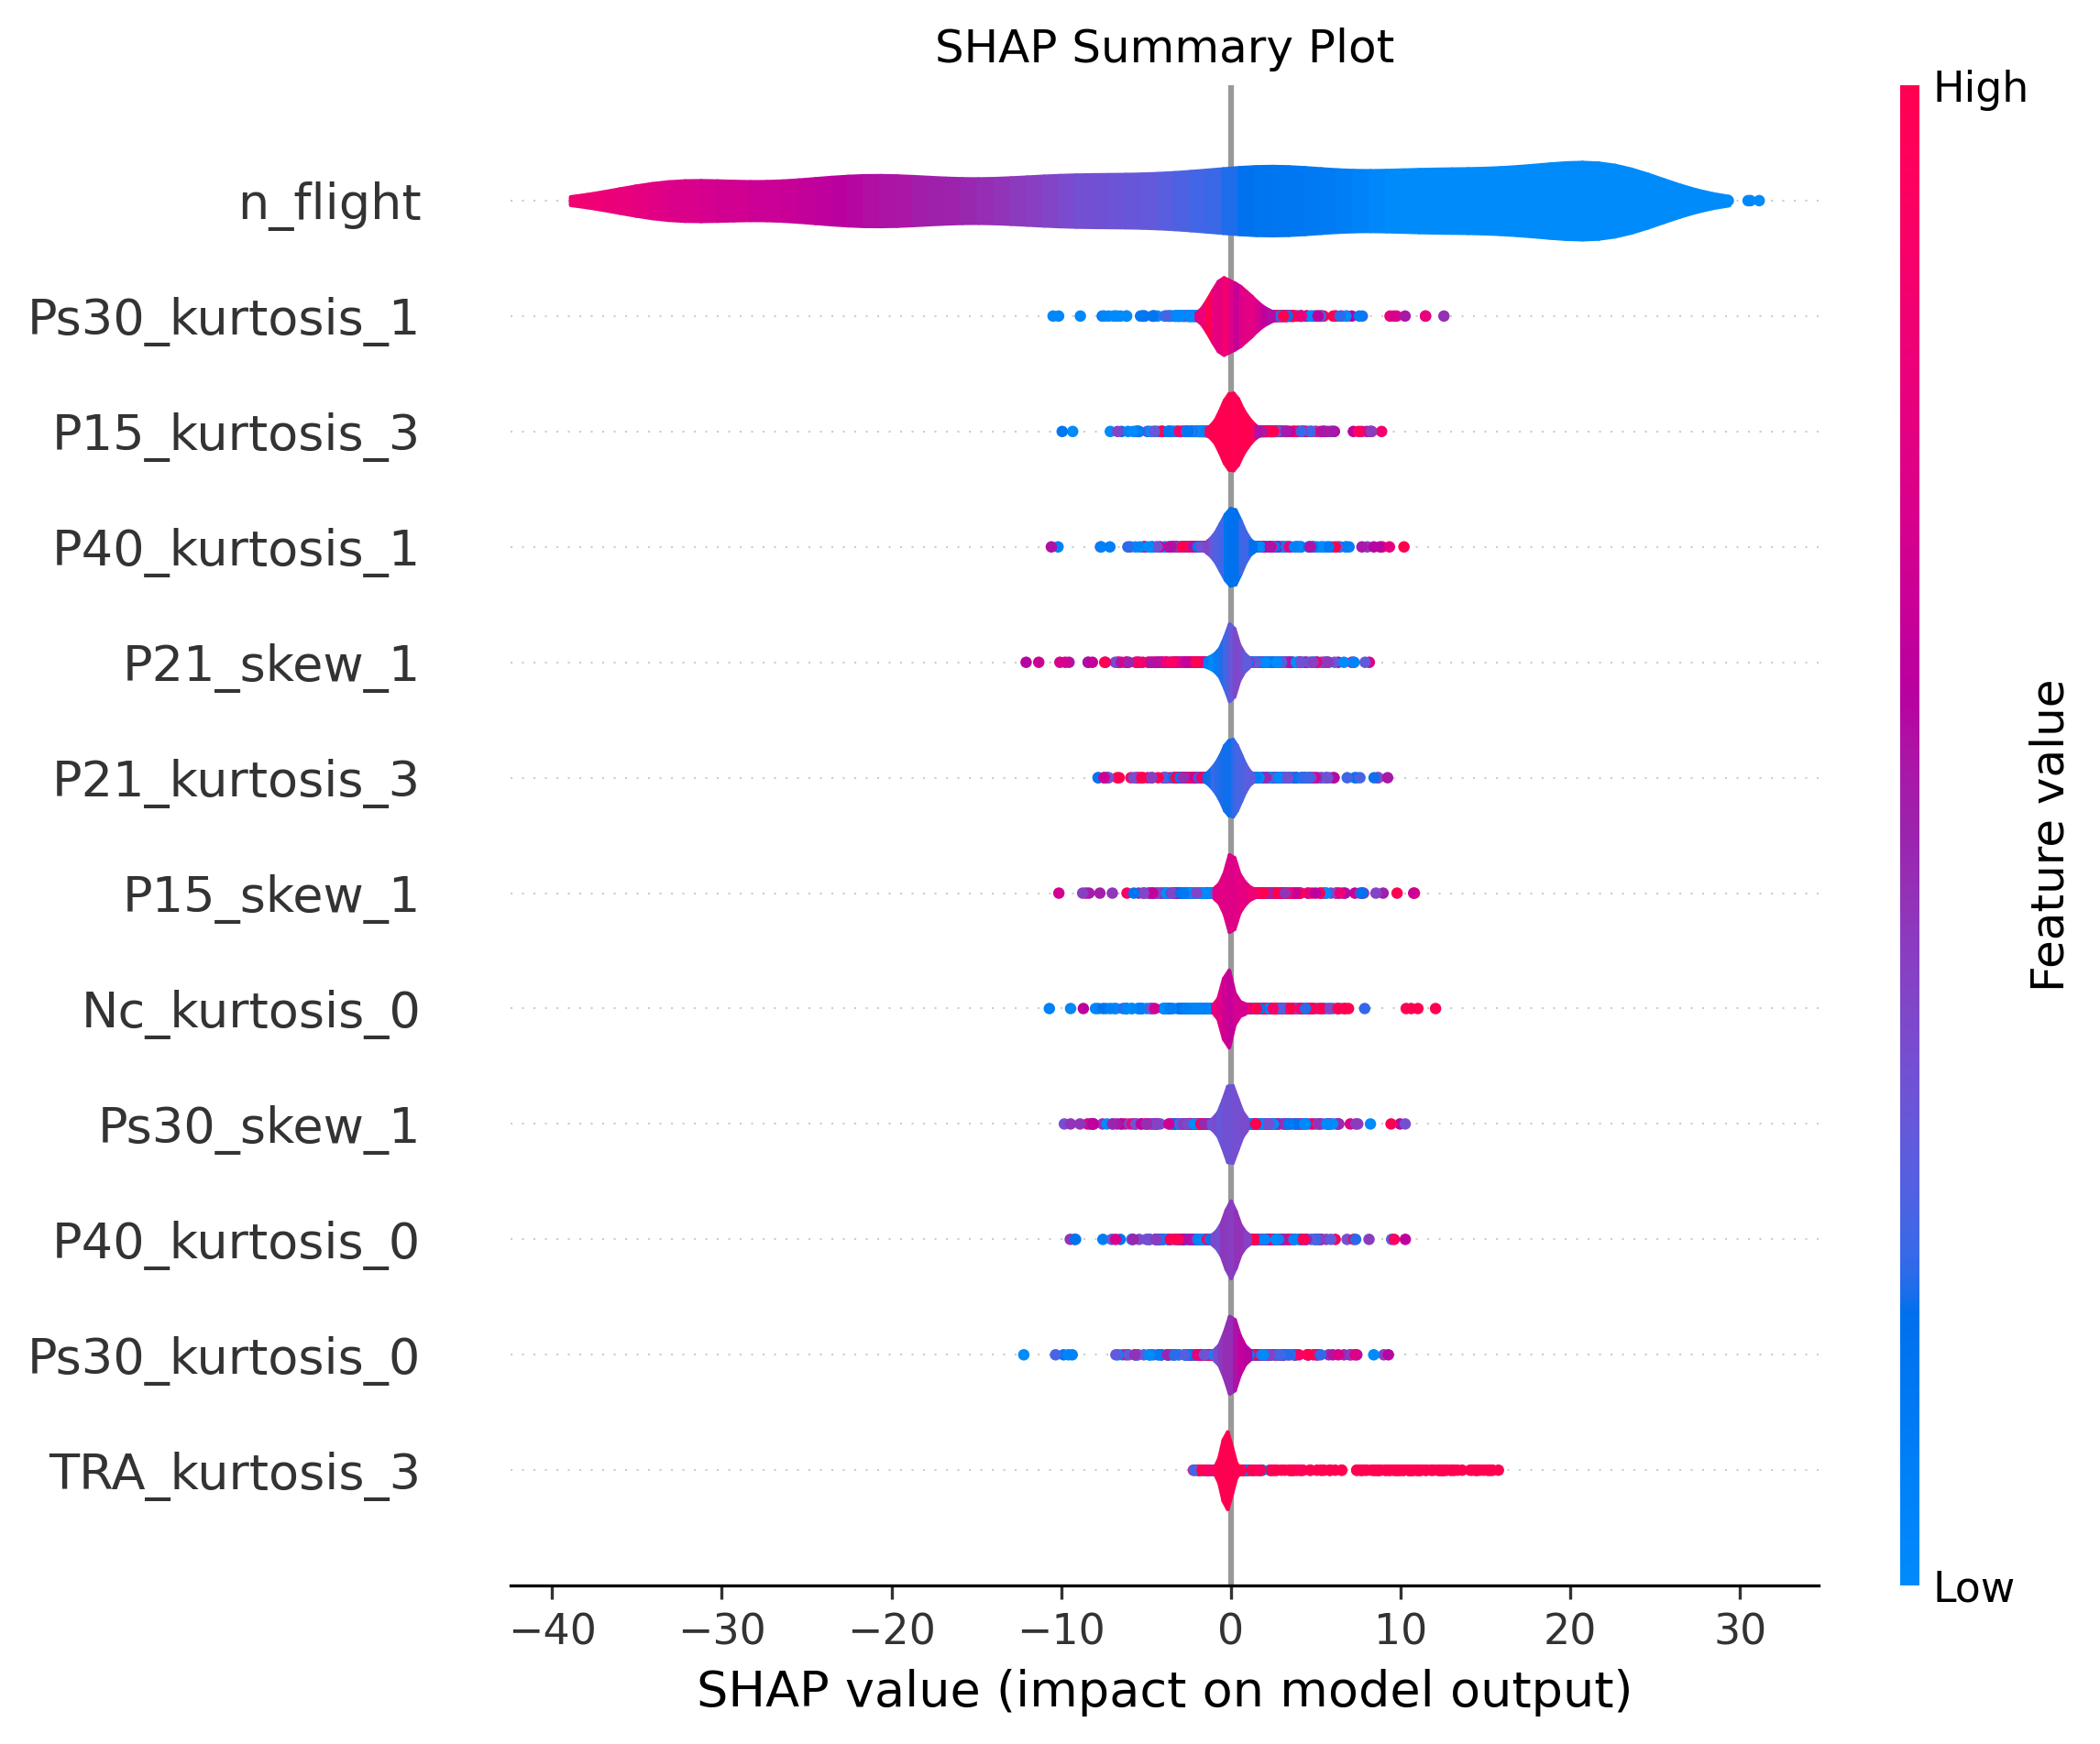
\includegraphics[scale=1.3]{figures/shap_summary.png}}}
            \caption{Example of RUL estimates produced and the Shapley Values for the predictions of the dataset}
        \end{figure}

    \end{block}

\end{column}

\separatorcolumn

\begin{column}{\smallcolwidth}

    \begin{block}{Discussion}

        \textit{Slight decrease in performance but much less compute time for training and inference.}
        \begin{table}
            \centering
            \begin{tabular}{ ccc }
                \toprule
                User & Model & Score \\
                \midrule
                IJoinedTooLate \cite{phm2021-1st-cnn} & Dilated CNN & 3.006 \\
                YellowJackets \cite{phm2021-2nd-inception} & Inception CNN & 3.327 \\
                DatrikUS \cite{phm2021-3rd-stacked-cnn} & Stacked DCNN & 3.651 \\
                \textbf{*} & \textbf{Bayesian Optimized XGBoost} & \textbf{5.687} \\
                \bottomrule
            \end{tabular}
            \caption{Comparison of model performances}
        \end{table}

    \end{block}

    \begin{block}{Conclusions}

        The research has delivered a comprehensive toolbox for systematic model optimization, showcasing performance enhancements over basic models but with a slight trade-off compared to Deep Learning methods.

        Future directions involve integrating segmentation algorithms into hyperparameter optimization, modifying feature selection techniques, and further experimentation with hyperparameter optimization processes. These endeavors contribute to the evolving landscape of predictive maintenance methodologies, striving for continuous improvements in both effectiveness and efficiency.

    \end{block}


    \begin{block}{References}

        \nocite{*}
        \footnotesize{\bibliographystyle{IEEEtran}\bibliography{poster.bib}}
    \end{block}

    \begin{block}{Further Information}
        Catch the Full Implementation and Code Details on GitHub! Scan the QR for in-depth insights and complete access to the implemented methodology and documentation.
        \begin{figure}
            \centering
            
\includegraphics[scale=0.9]{figures/frame.png}
        \end{figure}
    \end{block}

\end{column}

\separatorcolumn
\end{columns}
\end{frame}

\end{document}
